\documentclass[12pt,a4paper]{report}

% Packages
\usepackage[utf8]{inputenc}
\usepackage[T1]{fontenc}
\usepackage{geometry}
\geometry{a4paper, margin=1in}
\usepackage{graphicx}
\usepackage{xcolor}
\usepackage{tikz}
\usetikzlibrary{shapes.geometric, arrows, positioning, fit, calc, shadows.blur, patterns}
\usepackage{hyperref}
\usepackage{listings}
\usepackage{tcolorbox}
\usepackage{fancyhdr}
\usepackage{titlesec}
\usepackage{microtype}
\usepackage{enumitem}

% Setup Colors - Cyber Navy Theme
\definecolor{cyberblue}{RGB}{0, 71, 171}
\definecolor{cyberdark}{RGB}{10, 15, 20}
\definecolor{cybergreen}{RGB}{0, 255, 128}
\definecolor{cyberred}{RGB}{255, 60, 60}
\definecolor{codebg}{RGB}{245, 245, 245}

% Chapter Styling
\titleformat{\chapter}[display]
  {\normalfont\bfseries\color{cyberblue}}
  {\filleft\Large\chaptername\ \thechapter}
  {1ex}
  {\titlerule[2pt]\vspace{1ex}\huge\filleft}

% Setup Links
\hypersetup{
    colorlinks=true,
    linkcolor=cyberblue,
    urlcolor=cyberblue,
    pdftitle={cyberBOT CTF Engine - Detailed Field Manual},
}

% Setup Code Listings
\lstdefinestyle{bashstyle}{
    backgroundcolor=\color{codebg},
    basicstyle=\ttfamily\small,
    breakatwhitespace=false,         
    breaklines=true,                 
    captionpos=b,                    
    keepspaces=true,                 
    numbers=none,                    
    showspaces=false,                
    showstringspaces=false,
    showtabs=false,                  
    tabsize=2,
    frame=single,
    rulecolor=\color{lightgray}
}
\lstset{style=bashstyle}

% Header and Footer
\pagestyle{fancy}
\fancyhf{}
\fancyhead[L]{\textbf{cyberBOT CTF}}
\fancyhead[R]{Official Field Manual v3.5}
\fancyfoot[C]{\thepage}

% Custom Components
\newcommand{\cmd}[1]{\texttt{\color{cyberblue}\textbf{#1}}}
\newcommand{\note}[1]{
    \begin{tcolorbox}[colback=cyberblue!5, colframe=cyberblue, title=OPERATIONAL NOTE]
    #1
    \end{tcolorbox}
}
\newcommand{\warning}[1]{
    \begin{tcolorbox}[colback=cyberred!5, colframe=cyberred, title=CRITICAL WARNING]
    #1
    \end{tcolorbox}
}

% TikZ Styles
\tikzset{
    component/.style={rectangle, rounded corners, draw=cyberdark, fill=cyberblue!10, thick, minimum width=3.5cm, minimum height=1.2cm, text centered, font=\sffamily\small, blur shadow},
    database/.style={cylinder, shape border rotate=90, aspect=0.25, draw=cyberdark, fill=cybergreen!20, thick, minimum width=2.5cm, minimum height=2cm, text centered, font=\sffamily\small, blur shadow},
    process/.style={diamond, draw=cyberdark, fill=orange!20, thick, minimum width=3cm, minimum height=1cm, text centered, font=\sffamily\small, blur shadow},
    storage/.style={trapezium, draw=cyberdark, fill=gray!20, thick, minimum width=3cm, text centered, font=\sffamily\small, blur shadow},
    arrow/.style={thick, ->, >=stealth}
}

\begin{document}

% --- TITLE PAGE ---
\begin{titlepage}
    \centering
    \vspace*{2cm}
    \begin{tikzpicture}
        \node[circle, draw=cyberblue, line width=3pt, minimum size=4cm, fill=cyberdark, shadow blur] at (0,0) {
            \color{white}\huge\textbf{CB}
        };
        \draw[cyberblue, line width=2pt] (0,0) circle (2.3cm);
        \draw[cyberblue, line width=1pt, dashed] (0,0) circle (2.6cm);
        \foreach \a in {0,45,...,315}
            \draw[cyberblue, line width=1pt] (\a:2.6cm) -- (\a:3cm);
    \end{tikzpicture}
    
    \vspace{1.5cm}
    \Huge\textbf{\textsf{cyberBOT:}}\\
    \Huge\textbf{\textsf{CTF ENGINE MANUAL}}\\
    \vspace{0.8cm}
    \Large\textsf{Professional Asynchronous Discord CTF Operations}\\
    \vspace{2cm}
    \begin{tcolorbox}[colback=cyberdark, coltext=white, center, width=12cm]
        \centering \large PEAK ALIGNMENT \& DUAL-STREAM LOGGING EDITION
    \end{tcolorbox}
    \vfill
    \large \today\\
    \large Deployment-Ready Distribution
\end{titlepage}

\tableofcontents

% --- CHAPTER 1: SYSTEM INTRODUCTION ---
\chapter{System Introduction}
The \textbf{cyberBOT CTF Engine} is a high-performance Discord framework designed for competitive Capture The Flag events. Engineered for stability on both mobile (Termux) and desktop (Kali) hardware, it eliminates common database bottlenecks through a persistent asynchronous architecture.

\section{The Peak Architecture}
Traditional bots fail under load due to synchronous database operations. cyberBOT solves this by using:
\begin{itemize}
    \item \textbf{Persistent Database Connection:} A single, long-lived pipe to \cmd{bot.db} prevents "Connection Reset" errors.
    \item \textbf{WAL Mode:} Write-Ahead Logging allows participants to submit flags while the admin is simultaneously updating challenges.
    \item \textbf{Dual-Stream Logging:} Distinct monitoring for operational success vs. tactical failure.
\end{itemize}

\vspace{1cm}
\begin{center}
\textbf{Diagram 1.1: System Data Flow}\\
\vspace{0.5cm}
\begin{tikzpicture}[node distance=3cm, auto]
    \node (discord) [component, fill=indigo!10] {Discord API};
    \node (bot) [component, below=of discord] {cyberBOT Core};
    \node (db) [database, below=of bot] {bot.db (SQLite)};
    \node (storage) [storage, right=of db] {/uploads};
    
    \draw [arrow] (discord) -- node {Events} (bot);
    \draw [arrow] (bot) -- node {REST} (discord);
    \draw [arrow, dashed, cyberblue] (bot) -- node {Async WAL} (db);
    \draw [arrow] (bot) -- node {IO} (storage);
\end{tikzpicture}
\end{center}

% --- CHAPTER 2: HARDWARE & DEPLOYMENT ---
\chapter{Hardware \& Deployment}
cyberBOT is optimized for the constrained environments of rooted Android devices while maintaining full compatibility with Kali Linux.

\section{Pre-Flight Checklist}
\begin{enumerate}
    \item \textbf{Python 3.9+}: Required for advanced \texttt{asyncio} support.
    \item \textbf{SQLite3}: Pre-installed on most systems.
    \item \textbf{Intents}: Server Members, Presence, and Message Content must be enabled in the Discord Developer Portal.
\end{enumerate}

\section{Installation Protocols}
\begin{lstlisting}[language=bash, title=Standard Deployment]
# Clone and Setup
cd cyberBOT
python3 -m venv venv
source venv/bin/activate
pip install -r requirements.txt

# Configure Environment
cp .env.example .env
nano .env
\end{lstlisting}

\note{The \cmd{GUILD\_ID} variable is mandatory for \textbf{Instant Sync}. Global synchronization can take up to 60 minutes; Guild synchronization is instantaneous.}

% --- CHAPTER 3: ADMINISTRATIVE SETUP ---
\chapter{Administrative Setup}
Before mission deployment, the server's neurological pathways must be mapped via the \cmd{/setup} command.

\section{Initial Configuration}
Run \cmd{/setup} to link the following components:
\begin{itemize}
    \item \textbf{Leaderboard Channel:} Standings are updated here instantly on every score change.
    \item \textbf{Challenge Logs:} Real-time feed of successful captures and collusion alerts.
    \item \textbf{Wrong Submissions:} Tracks every failed attempt, including the exact string entered by the player.
    \item \textbf{Champion Role:} Strictly assigned to the \#1 ranked agent.
\end{itemize}

\section{Recursive Point Economics}
The engine ensures a fair environment by tracking every point transaction. If an administrator deletes a challenge or a hint, the bot calculates the refunds and restores the points to all affected users instantly.

\vspace{1cm}
\begin{center}
\textbf{Diagram 3.1: Recursive Refund Flow}\\
\vspace{0.5cm}
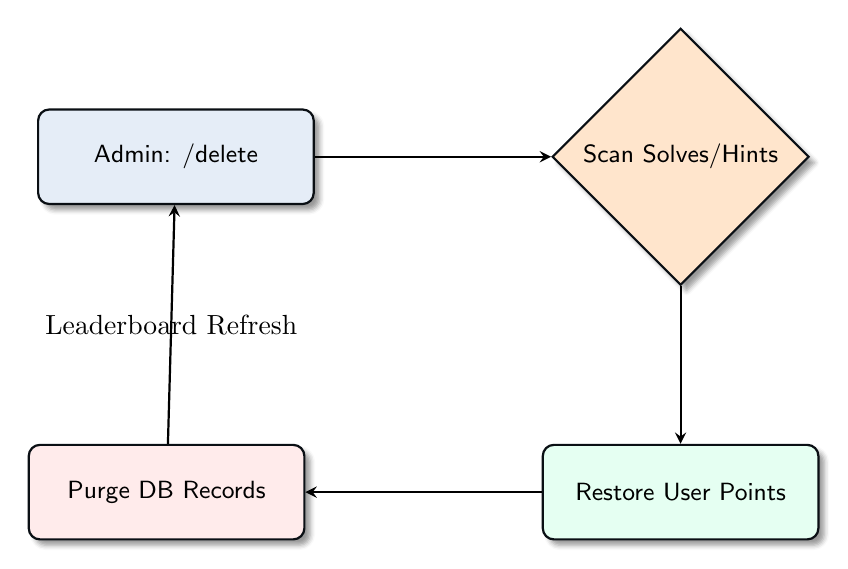
\begin{tikzpicture}[node distance=2cm]
    \node (admin) [component] {Admin: /delete};
    \node (check) [process, right=of admin, xshift=1cm] {Scan Solves/Hints};
    \node (refund) [component, below=of check, fill=cybergreen!10] {Restore User Points};
    \node (wipe) [component, left=of refund, xshift=-1cm, fill=cyberred!10] {Purge DB Records};

    \draw [arrow] (admin) -- (check);
    \draw [arrow] (check) -- (refund);
    \draw [arrow] (refund) -- (wipe);
    \draw [arrow] (wipe) -- node {Leaderboard Refresh} (admin);
\end{tikzpicture}
\end{center}

% --- CHAPTER 4: MISSION SCHEDULING ---
\chapter{Mission Scheduling}
cyberBOT features a "Set and Forget" scheduler, allowing for entire CTF events to be pre-programmed.

\section{The Scheduler Engine}
When a challenge is posted with a future \cmd{start\_time}, the bot:
\begin{enumerate}
    \item Saves mission metadata to \cmd{bot.db}.
    \item Stores any attached files in the \cmd{/uploads} directory.
    \item Triggers \cmd{check\_pending\_posts} every 60 seconds.
\end{enumerate}

\vspace{1cm}
\begin{center}
\textbf{Diagram 4.1: Scheduled Posting Logic}\\
\vspace{0.5cm}
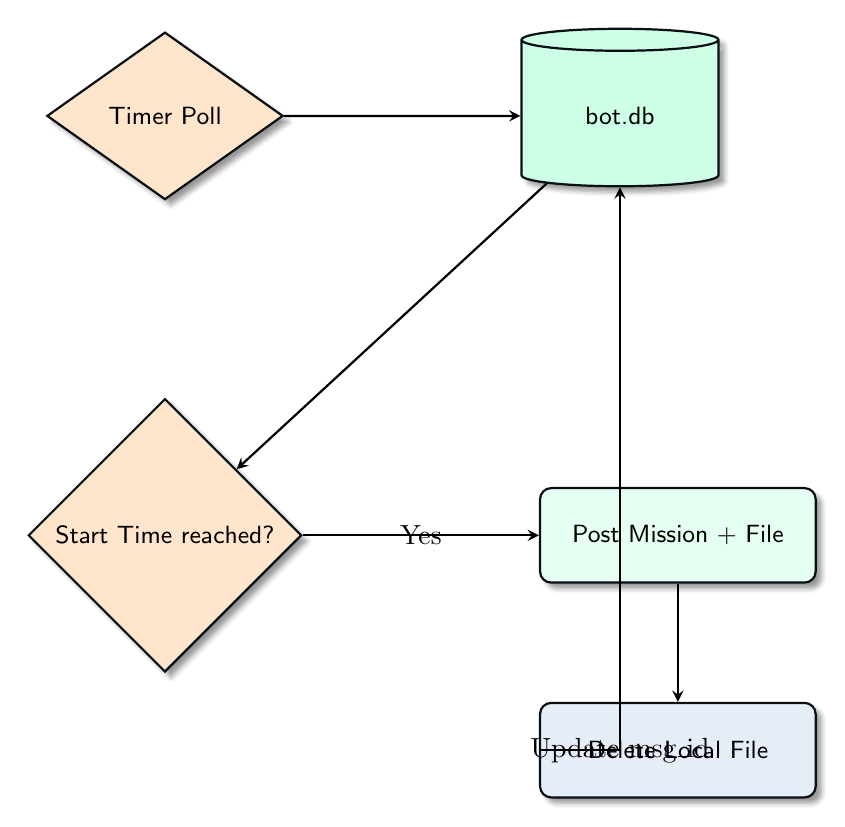
\begin{tikzpicture}[node distance=1.5cm]
    \node (start) [process] {Timer Poll};
    \node (db) [database, right=of start, xshift=1.5cm] {bot.db};
    \node (found) [process, below=of start, yshift=-1cm] {Start Time reached?};
    \node (post) [component, right=of found, xshift=1.5cm, fill=cybergreen!10] {Post Mission + File};
    \node (clean) [component, below=of post] {Delete Local File};

    \draw [arrow] (start) -- (db);
    \draw [arrow] (db) -- (found);
    \draw [arrow] (found) -- node {Yes} (post);
    \draw [arrow] (post) -- (clean);
    \draw [arrow] (clean) -| node {Update msg\_id} (db);
\end{tikzpicture}
\end{center}

\section{Anti-Deletion Watchdog}
Every 60 seconds, the engine performs a heartbeat check on every active mission. cyberBOT monitors **both** the mission embed and the file attachment message. 

\begin{center}
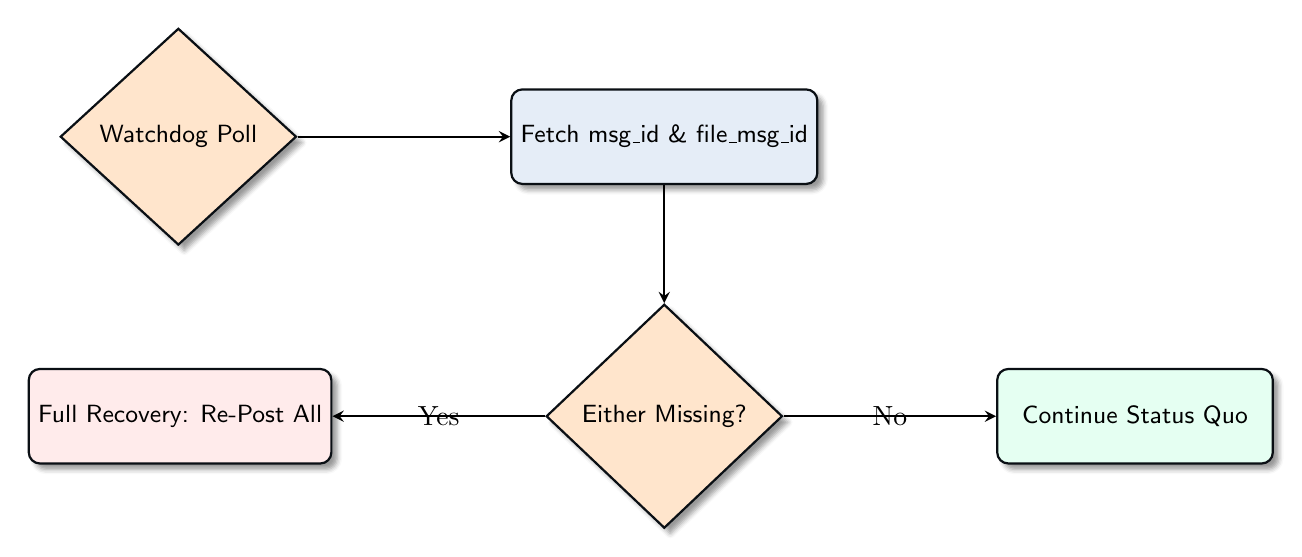
\begin{tikzpicture}[node distance=1.5cm]
    \node (task) [process] {Watchdog Poll};
    \node (check) [component, right=of task, xshift=1.2cm] {Fetch msg\_id \& file\_msg\_id};
    \node (exists) [process, below=of check] {Either Missing?};
    \node (ok) [component, right=of exists, xshift=1.2cm, fill=cybergreen!10] {Continue Status Quo};
    \node (repost) [component, left=of exists, xshift=-1.2cm, fill=cyberred!10] {Full Recovery: Re-Post All};

    \draw [arrow] (task) -- (check);
    \draw [arrow] (check) -- (exists);
    \draw [arrow] (exists) -- node {No} (ok);
    \draw [arrow] (exists) -- node {Yes} (repost);
\end{tikzpicture}
\end{center}

If either message is deleted, the bot performs a **Full Clean Recovery**:
\begin{enumerate}
    \item Attempts to delete the remaining message fragment (if any) to prevent channel clutter.
    \item Re-posts the mission embed instantly.
    \item Re-attaches the mission file from local storage.
    \item Synchronizes the new message IDs in the persistent database.
\end{enumerate}

% --- CHAPTER 5: AGENT PROMOTION SYSTEM ---
\chapter{Agent Promotion System}
The promotion engine is fully dynamic, allowing administrators to define an unlimited number of rank roles.

\section{Defining Ranks}
Use \cmd{/set\_rank\_role} to link any role to a point threshold. 
\begin{itemize}
    \item \cmd{Novice} $\rightarrow$ 500 pts
    \item \cmd{Elite} $\rightarrow$ 5000 pts
    \item \cmd{God} $\rightarrow$ 10000 pts
\end{itemize}

\vspace{1cm}
\begin{center}
\textbf{Diagram 5.1: Dynamic Promotion Flow}\\
\vspace{0.5cm}
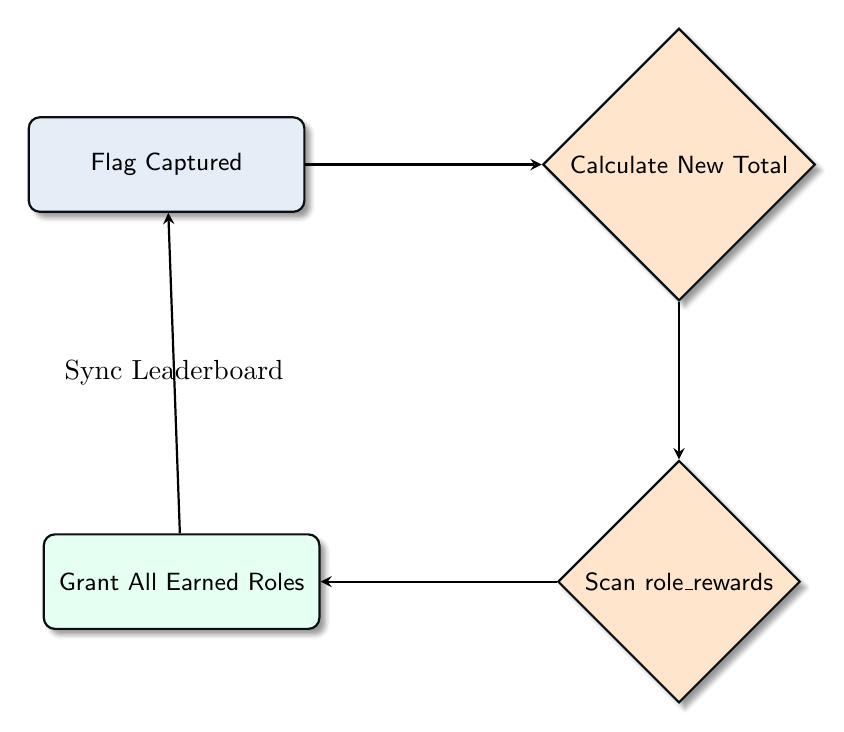
\begin{tikzpicture}[node distance=2cm]
    \node (solve) [component] {Flag Captured};
    \node (calc) [process, right=of solve, xshift=1cm] {Calculate New Total};
    \node (scan) [process, below=of calc] {Scan role\_rewards};
    \node (assign) [component, left=of scan, xshift=-1cm, fill=cybergreen!10] {Grant All Earned Roles};

    \draw [arrow] (solve) -- (calc);
    \draw [arrow] (calc) -- (scan);
    \draw [arrow] (scan) -- (assign);
    \draw [arrow] (assign) -- node {Sync Leaderboard} (solve);
\end{tikzpicture}
\end{center}

% --- CHAPTER 6: VISUAL IDENTIFICATION ---
\chapter{Visual Identification}
cyberBOT uses the Python Imaging Library (PIL) to generate high-resolution Agent ID cards.

\section{The Champion's Visual Identity}
The \#1 ranked player on the leaderboard is granted the **"Golden Protocol"** visual theme. This is automatically applied to their ID card whenever they run \cmd{/profile}.

\begin{itemize}
    \item \textbf{Gold Aesthetic:} The primary border, accents, and stat-box outlines shift to high-visibility Gold (\texttt{\#FFD700}).
    \item \textbf{Geometric Shift:} The standard circular rank icon is replaced with a **Diamond** glyph, signifying their status at the peak of the standings.
    \item \textbf{Unique Designation:} The primary badge title is locked to \cmd{CHAMPION}.
    \item \textbf{Enhanced Contrast:} A deeper shadow-cast is applied to the avatar ring to make the golden elements appear to glow.
\end{itemize}

\vspace{1cm}
\begin{center}
\textbf{Diagram 6.2: The Golden Protocol (Champion Visuals)}\\
\vspace{0.5cm}
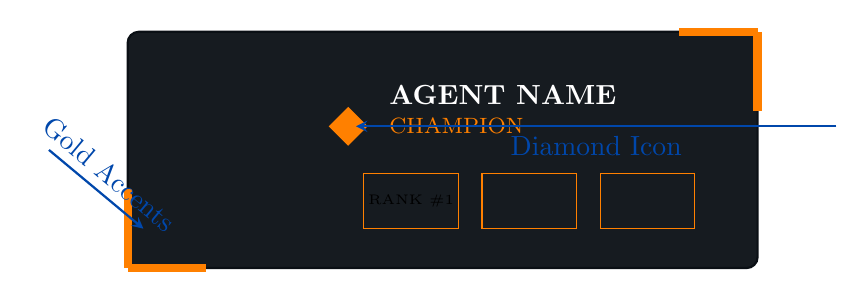
\begin{tikzpicture}
    % Represent the Card
    \draw[cyberdark, fill=cyberdark!95, rounded corners, thick] (0,0) rectangle (8,3);
    
    % Golden Accents
    \draw[orange, line width=3pt] (0,0) -- (1,0);
    \draw[orange, line width=3pt] (0,0) -- (0,1);
    \draw[orange, line width=3pt] (8,3) -- (7,3);
    \draw[orange, line width=3pt] (8,3) -- (8,2);
    
    % Diamond Icon
    \node[diamond, fill=orange, minimum size=0.5cm] at (2.8, 1.8) {};
    
    % Text Placeholders
    \node[anchor=west, white] at (3.2, 2.2) {\textbf{AGENT NAME}};
    \node[anchor=west, orange] at (3.2, 1.8) {\footnotesize CHAMPION};
    
    % Stat Boxes
    \draw[orange, thin] (3, 0.5) rectangle (4.2, 1.2);
    \draw[orange, thin] (4.5, 0.5) rectangle (5.7, 1.2);
    \draw[orange, thin] (6, 0.5) rectangle (7.2, 1.2);
    
    \node at (3.6, 0.85) {\tiny RANK \#1};
    
    % Annotation
    \draw[arrow, cyberblue] (-1, 1.5) -- node[anchor=south, sloped] {Gold Accents} (0.2, 0.5);
    \draw[arrow, cyberblue] (9, 1.8) -- node[anchor=north, sloped] {Diamond Icon} (2.9, 1.8);
\end{tikzpicture}
\end{center}

\section{Automatic Promotion Logic}
The engine monitors the standings instantly. When an Agent overtakes the current \#1 player, cyberBOT:
\begin{enumerate}
    \item Strips the Champion Role from the previous holder.
    \item Grants the Champion Role to the new winner.
    \item Broadcasts a "Belt Stolen" announcement in the General Channel.
    \item Immediately enables the Golden Protocol for the new winner's profile card.
\end{enumerate}

% --- CHAPTER 7: SECURITY & MAINTENANCE ---
\chapter{Security \& Maintenance}
Maintaining the integrity of the CTF database is the highest priority.

\section{Millisecond Tie-Breaking}
Scores are sorted by \cmd{points DESC} and then by \cmd{timestamp ASC}. Since timestamps are stored as \texttt{REAL} floats (millisecond precision), the person who submits first is mathematically guaranteed the higher rank.

\section{Live-Swap Imports}
The \cmd{/import} command allows for a database restoration without turning off the bot. This is critical for preventing downtime during an active competition.

\vspace{2cm}
\begin{center}
\textbf{--- END OF FIELD MANUAL ---}\\
\textit{cyberBOT: High-Performance Discord CTF Engine}
\end{center}

\end{document}
